% Created by tikzDevice version 0.7.0 on 2014-07-29 12:43:57
% !TEX encoding = UTF-8 Unicode
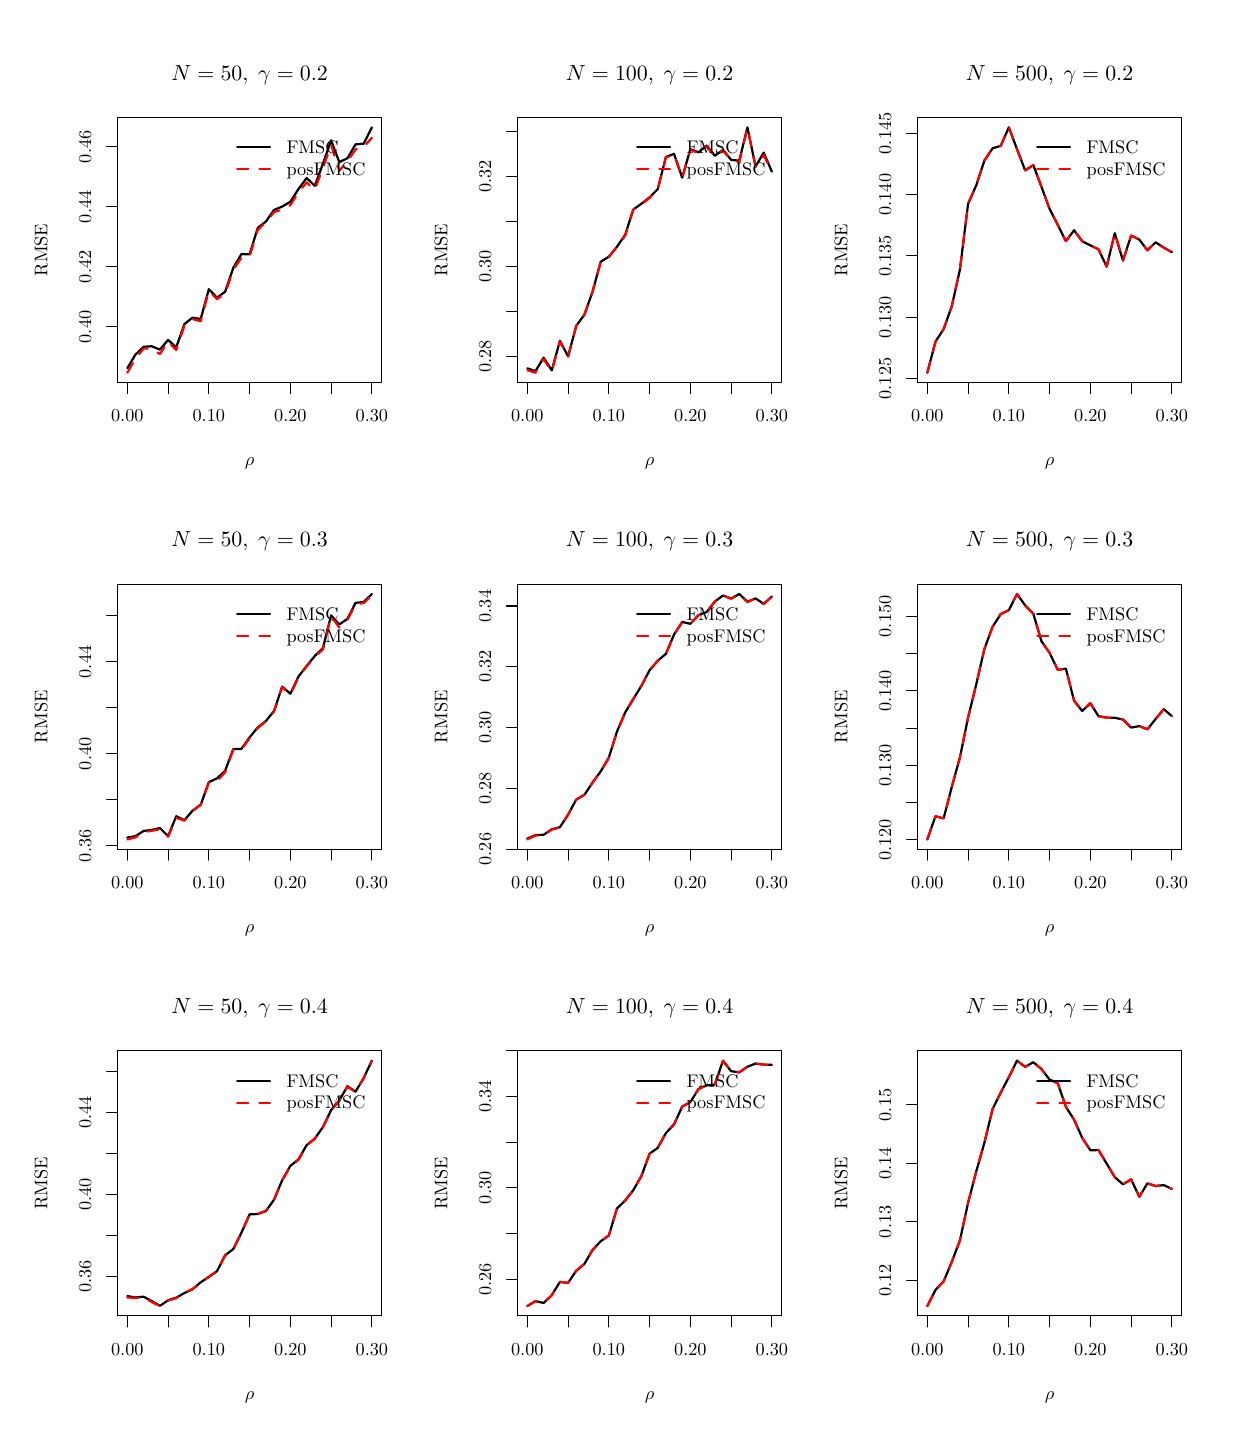
\begin{tikzpicture}[x=1pt,y=1pt]
\definecolor[named]{fillColor}{rgb}{1.00,1.00,1.00}
\path[use as bounding box,fill=fillColor,fill opacity=0.00] (0,0) rectangle (433.62,505.89);
\begin{scope}
\path[clip] ( 32.47,377.65) rectangle (127.91,473.42);
\definecolor[named]{drawColor}{rgb}{0.00,0.00,0.00}

\path[draw=drawColor,line width= 0.8pt,line join=round,line cap=round] ( 36.01,382.83) --
	( 38.95,387.77) --
	( 41.90,390.58) --
	( 44.84,390.76) --
	( 47.79,389.54) --
	( 50.73,393.05) --
	( 53.68,390.37) --
	( 56.63,398.76) --
	( 59.57,401.11) --
	( 62.52,400.61) --
	( 65.46,411.39) --
	( 68.41,408.34) --
	( 71.35,410.47) --
	( 74.30,419.12) --
	( 77.24,424.08) --
	( 80.19,423.97) --
	( 83.14,433.52) --
	( 86.08,435.83) --
	( 89.03,440.02) --
	( 91.97,441.24) --
	( 94.92,442.98) --
	( 97.86,447.59) --
	(100.81,451.55) --
	(103.75,448.74) --
	(106.70,456.75) --
	(109.65,465.17) --
	(112.59,457.33) --
	(115.54,458.69) --
	(118.48,463.72) --
	(121.43,463.97) --
	(124.37,469.87);
\end{scope}
\begin{scope}
\path[clip] (  0.00,  0.00) rectangle (433.62,505.89);
\definecolor[named]{drawColor}{rgb}{0.00,0.00,0.00}

\path[draw=drawColor,line width= 0.4pt,line join=round,line cap=round] ( 36.01,377.65) -- (124.37,377.65);

\path[draw=drawColor,line width= 0.4pt,line join=round,line cap=round] ( 36.01,377.65) -- ( 36.01,373.69);

\path[draw=drawColor,line width= 0.4pt,line join=round,line cap=round] ( 50.73,377.65) -- ( 50.73,373.69);

\path[draw=drawColor,line width= 0.4pt,line join=round,line cap=round] ( 65.46,377.65) -- ( 65.46,373.69);

\path[draw=drawColor,line width= 0.4pt,line join=round,line cap=round] ( 80.19,377.65) -- ( 80.19,373.69);

\path[draw=drawColor,line width= 0.4pt,line join=round,line cap=round] ( 94.92,377.65) -- ( 94.92,373.69);

\path[draw=drawColor,line width= 0.4pt,line join=round,line cap=round] (109.65,377.65) -- (109.65,373.69);

\path[draw=drawColor,line width= 0.4pt,line join=round,line cap=round] (124.37,377.65) -- (124.37,373.69);

\node[text=drawColor,anchor=base,inner sep=0pt, outer sep=0pt, scale=  0.66] at ( 36.01,363.40) {0.00};

\node[text=drawColor,anchor=base,inner sep=0pt, outer sep=0pt, scale=  0.66] at ( 65.46,363.40) {0.10};

\node[text=drawColor,anchor=base,inner sep=0pt, outer sep=0pt, scale=  0.66] at ( 94.92,363.40) {0.20};

\node[text=drawColor,anchor=base,inner sep=0pt, outer sep=0pt, scale=  0.66] at (124.37,363.40) {0.30};

\path[draw=drawColor,line width= 0.4pt,line join=round,line cap=round] ( 32.47,397.76) -- ( 32.47,462.81);

\path[draw=drawColor,line width= 0.4pt,line join=round,line cap=round] ( 32.47,397.76) -- ( 28.51,397.76);

\path[draw=drawColor,line width= 0.4pt,line join=round,line cap=round] ( 32.47,419.45) -- ( 28.51,419.45);

\path[draw=drawColor,line width= 0.4pt,line join=round,line cap=round] ( 32.47,441.13) -- ( 28.51,441.13);

\path[draw=drawColor,line width= 0.4pt,line join=round,line cap=round] ( 32.47,462.81) -- ( 28.51,462.81);

\node[text=drawColor,rotate= 90.00,anchor=base,inner sep=0pt, outer sep=0pt, scale=  0.66] at ( 22.97,397.76) {0.40};

\node[text=drawColor,rotate= 90.00,anchor=base,inner sep=0pt, outer sep=0pt, scale=  0.66] at ( 22.97,419.45) {0.42};

\node[text=drawColor,rotate= 90.00,anchor=base,inner sep=0pt, outer sep=0pt, scale=  0.66] at ( 22.97,441.13) {0.44};

\node[text=drawColor,rotate= 90.00,anchor=base,inner sep=0pt, outer sep=0pt, scale=  0.66] at ( 22.97,462.81) {0.46};

\path[draw=drawColor,line width= 0.4pt,line join=round,line cap=round] ( 32.47,377.65) --
	(127.91,377.65) --
	(127.91,473.42) --
	( 32.47,473.42) --
	( 32.47,377.65);
\end{scope}
\begin{scope}
\path[clip] (  0.00,337.26) rectangle (144.54,505.89);
\definecolor[named]{drawColor}{rgb}{0.00,0.00,0.00}

\node[text=drawColor,anchor=base,inner sep=0pt, outer sep=0pt, scale=  0.79] at ( 80.19,486.92) {\bfseries $N=50, \;\gamma=0.2$};

\node[text=drawColor,anchor=base,inner sep=0pt, outer sep=0pt, scale=  0.66] at ( 80.19,347.56) {$\rho$};

\node[text=drawColor,rotate= 90.00,anchor=base,inner sep=0pt, outer sep=0pt, scale=  0.66] at (  7.13,425.53) {RMSE};
\end{scope}
\begin{scope}
\path[clip] ( 32.47,377.65) rectangle (127.91,473.42);
\definecolor[named]{drawColor}{rgb}{1.00,0.00,0.00}

\path[draw=drawColor,line width= 0.8pt,dash pattern=on 4pt off 4pt ,line join=round,line cap=round] ( 36.01,381.20) --
	( 38.95,386.30) --
	( 41.90,389.99) --
	( 44.84,389.79) --
	( 47.79,387.95) --
	( 50.73,392.49) --
	( 53.68,389.40) --
	( 56.63,398.22) --
	( 59.57,400.59) --
	( 62.52,399.81) --
	( 65.46,410.74) --
	( 68.41,407.80) --
	( 71.35,409.74) --
	( 74.30,418.46) --
	( 77.24,422.74) --
	( 80.19,423.26) --
	( 83.14,432.77) --
	( 86.08,435.64) --
	( 89.03,439.24) --
	( 91.97,440.21) --
	( 94.92,441.75) --
	( 97.86,446.39) --
	(100.81,449.97) --
	(103.75,447.31) --
	(106.70,455.25) --
	(109.65,463.64) --
	(112.59,454.14) --
	(115.54,457.66) --
	(118.48,461.87) --
	(121.43,462.78) --
	(124.37,466.09);
\definecolor[named]{drawColor}{rgb}{0.00,0.00,0.00}

\path[draw=drawColor,line width= 0.8pt,line join=round,line cap=round] ( 75.72,462.63) -- ( 87.60,462.63);
\definecolor[named]{drawColor}{rgb}{1.00,0.00,0.00}

\path[draw=drawColor,line width= 0.8pt,dash pattern=on 4pt off 4pt ,line join=round,line cap=round] ( 75.72,454.71) -- ( 87.60,454.71);
\definecolor[named]{drawColor}{rgb}{0.00,0.00,0.00}

\node[text=drawColor,anchor=base west,inner sep=0pt, outer sep=0pt, scale=  0.66] at ( 93.54,460.35) {FMSC};

\node[text=drawColor,anchor=base west,inner sep=0pt, outer sep=0pt, scale=  0.66] at ( 93.54,452.43) {posFMSC};
\end{scope}
\begin{scope}
\path[clip] (177.01,377.65) rectangle (272.45,473.42);
\definecolor[named]{drawColor}{rgb}{0.00,0.00,0.00}

\path[draw=drawColor,line width= 0.8pt,line join=round,line cap=round] (180.55,382.79) --
	(183.49,381.78) --
	(186.44,386.65) --
	(189.38,382.04) --
	(192.33,392.73) --
	(195.27,387.11) --
	(198.22,398.14) --
	(201.17,402.20) --
	(204.11,410.45) --
	(207.06,421.30) --
	(210.00,423.12) --
	(212.95,426.74) --
	(215.89,430.99) --
	(218.84,440.18) --
	(221.78,442.26) --
	(224.73,444.55) --
	(227.68,447.57) --
	(230.62,459.17) --
	(233.57,460.27) --
	(236.51,451.70) --
	(239.46,461.98) --
	(242.40,460.84) --
	(245.35,463.30) --
	(248.29,459.60) --
	(251.24,461.71) --
	(254.19,458.14) --
	(257.13,457.81) --
	(260.08,469.87) --
	(263.02,455.74) --
	(265.97,460.74) --
	(268.91,453.86);
\end{scope}
\begin{scope}
\path[clip] (  0.00,  0.00) rectangle (433.62,505.89);
\definecolor[named]{drawColor}{rgb}{0.00,0.00,0.00}

\path[draw=drawColor,line width= 0.4pt,line join=round,line cap=round] (180.55,377.65) -- (268.91,377.65);

\path[draw=drawColor,line width= 0.4pt,line join=round,line cap=round] (180.55,377.65) -- (180.55,373.69);

\path[draw=drawColor,line width= 0.4pt,line join=round,line cap=round] (195.27,377.65) -- (195.27,373.69);

\path[draw=drawColor,line width= 0.4pt,line join=round,line cap=round] (210.00,377.65) -- (210.00,373.69);

\path[draw=drawColor,line width= 0.4pt,line join=round,line cap=round] (224.73,377.65) -- (224.73,373.69);

\path[draw=drawColor,line width= 0.4pt,line join=round,line cap=round] (239.46,377.65) -- (239.46,373.69);

\path[draw=drawColor,line width= 0.4pt,line join=round,line cap=round] (254.19,377.65) -- (254.19,373.69);

\path[draw=drawColor,line width= 0.4pt,line join=round,line cap=round] (268.91,377.65) -- (268.91,373.69);

\node[text=drawColor,anchor=base,inner sep=0pt, outer sep=0pt, scale=  0.66] at (180.55,363.40) {0.00};

\node[text=drawColor,anchor=base,inner sep=0pt, outer sep=0pt, scale=  0.66] at (210.00,363.40) {0.10};

\node[text=drawColor,anchor=base,inner sep=0pt, outer sep=0pt, scale=  0.66] at (239.46,363.40) {0.20};

\node[text=drawColor,anchor=base,inner sep=0pt, outer sep=0pt, scale=  0.66] at (268.91,363.40) {0.30};

\path[draw=drawColor,line width= 0.4pt,line join=round,line cap=round] (177.01,387.04) -- (177.01,468.48);

\path[draw=drawColor,line width= 0.4pt,line join=round,line cap=round] (177.01,387.04) -- (173.05,387.04);

\path[draw=drawColor,line width= 0.4pt,line join=round,line cap=round] (177.01,403.33) -- (173.05,403.33);

\path[draw=drawColor,line width= 0.4pt,line join=round,line cap=round] (177.01,419.62) -- (173.05,419.62);

\path[draw=drawColor,line width= 0.4pt,line join=round,line cap=round] (177.01,435.91) -- (173.05,435.91);

\path[draw=drawColor,line width= 0.4pt,line join=round,line cap=round] (177.01,452.19) -- (173.05,452.19);

\path[draw=drawColor,line width= 0.4pt,line join=round,line cap=round] (177.01,468.48) -- (173.05,468.48);

\node[text=drawColor,rotate= 90.00,anchor=base,inner sep=0pt, outer sep=0pt, scale=  0.66] at (167.51,387.04) {0.28};

\node[text=drawColor,rotate= 90.00,anchor=base,inner sep=0pt, outer sep=0pt, scale=  0.66] at (167.51,419.62) {0.30};

\node[text=drawColor,rotate= 90.00,anchor=base,inner sep=0pt, outer sep=0pt, scale=  0.66] at (167.51,452.19) {0.32};

\path[draw=drawColor,line width= 0.4pt,line join=round,line cap=round] (177.01,377.65) --
	(272.45,377.65) --
	(272.45,473.42) --
	(177.01,473.42) --
	(177.01,377.65);
\end{scope}
\begin{scope}
\path[clip] (144.54,337.26) rectangle (289.08,505.89);
\definecolor[named]{drawColor}{rgb}{0.00,0.00,0.00}

\node[text=drawColor,anchor=base,inner sep=0pt, outer sep=0pt, scale=  0.79] at (224.73,486.92) {\bfseries $N=100, \;\gamma=0.2$};

\node[text=drawColor,anchor=base,inner sep=0pt, outer sep=0pt, scale=  0.66] at (224.73,347.56) {$\rho$};

\node[text=drawColor,rotate= 90.00,anchor=base,inner sep=0pt, outer sep=0pt, scale=  0.66] at (151.67,425.53) {RMSE};
\end{scope}
\begin{scope}
\path[clip] (177.01,377.65) rectangle (272.45,473.42);
\definecolor[named]{drawColor}{rgb}{1.00,0.00,0.00}

\path[draw=drawColor,line width= 0.8pt,dash pattern=on 4pt off 4pt ,line join=round,line cap=round] (180.55,382.12) --
	(183.49,381.20) --
	(186.44,386.14) --
	(189.38,381.63) --
	(192.33,392.49) --
	(195.27,386.83) --
	(198.22,398.11) --
	(201.17,402.12) --
	(204.11,410.48) --
	(207.06,421.22) --
	(210.00,423.06) --
	(212.95,426.62) --
	(215.89,430.71) --
	(218.84,440.19) --
	(221.78,441.98) --
	(224.73,444.41) --
	(227.68,447.49) --
	(230.62,458.97) --
	(233.57,460.04) --
	(236.51,451.53) --
	(239.46,461.79) --
	(242.40,460.48) --
	(245.35,462.96) --
	(248.29,459.35) --
	(251.24,461.60) --
	(254.19,457.93) --
	(257.13,457.37) --
	(260.08,469.60) --
	(263.02,455.61) --
	(265.97,459.78) --
	(268.91,453.82);
\definecolor[named]{drawColor}{rgb}{0.00,0.00,0.00}

\path[draw=drawColor,line width= 0.8pt,line join=round,line cap=round] (220.26,462.63) -- (232.14,462.63);
\definecolor[named]{drawColor}{rgb}{1.00,0.00,0.00}

\path[draw=drawColor,line width= 0.8pt,dash pattern=on 4pt off 4pt ,line join=round,line cap=round] (220.26,454.71) -- (232.14,454.71);
\definecolor[named]{drawColor}{rgb}{0.00,0.00,0.00}

\node[text=drawColor,anchor=base west,inner sep=0pt, outer sep=0pt, scale=  0.66] at (238.08,460.35) {FMSC};

\node[text=drawColor,anchor=base west,inner sep=0pt, outer sep=0pt, scale=  0.66] at (238.08,452.43) {posFMSC};
\end{scope}
\begin{scope}
\path[clip] (321.55,377.65) rectangle (416.99,473.42);
\definecolor[named]{drawColor}{rgb}{0.00,0.00,0.00}

\path[draw=drawColor,line width= 0.8pt,line join=round,line cap=round] (325.09,381.20) --
	(328.03,392.44) --
	(330.98,396.99) --
	(333.92,405.21) --
	(336.87,418.47) --
	(339.81,442.22) --
	(342.76,448.92) --
	(345.71,457.86) --
	(348.65,462.29) --
	(351.60,463.17) --
	(354.54,469.87) --
	(357.49,461.99) --
	(360.43,454.31) --
	(363.38,456.21) --
	(366.32,448.42) --
	(369.27,440.38) --
	(372.22,434.62) --
	(375.16,428.75) --
	(378.11,432.68) --
	(381.05,428.71) --
	(384.00,427.22) --
	(386.94,425.79) --
	(389.89,419.54) --
	(392.83,431.63) --
	(395.78,421.70) --
	(398.73,430.77) --
	(401.67,429.32) --
	(404.62,425.43) --
	(407.56,428.32) --
	(410.51,426.42) --
	(413.45,424.76);
\end{scope}
\begin{scope}
\path[clip] (  0.00,  0.00) rectangle (433.62,505.89);
\definecolor[named]{drawColor}{rgb}{0.00,0.00,0.00}

\path[draw=drawColor,line width= 0.4pt,line join=round,line cap=round] (325.09,377.65) -- (413.45,377.65);

\path[draw=drawColor,line width= 0.4pt,line join=round,line cap=round] (325.09,377.65) -- (325.09,373.69);

\path[draw=drawColor,line width= 0.4pt,line join=round,line cap=round] (339.81,377.65) -- (339.81,373.69);

\path[draw=drawColor,line width= 0.4pt,line join=round,line cap=round] (354.54,377.65) -- (354.54,373.69);

\path[draw=drawColor,line width= 0.4pt,line join=round,line cap=round] (369.27,377.65) -- (369.27,373.69);

\path[draw=drawColor,line width= 0.4pt,line join=round,line cap=round] (384.00,377.65) -- (384.00,373.69);

\path[draw=drawColor,line width= 0.4pt,line join=round,line cap=round] (398.73,377.65) -- (398.73,373.69);

\path[draw=drawColor,line width= 0.4pt,line join=round,line cap=round] (413.45,377.65) -- (413.45,373.69);

\node[text=drawColor,anchor=base,inner sep=0pt, outer sep=0pt, scale=  0.66] at (325.09,363.40) {0.00};

\node[text=drawColor,anchor=base,inner sep=0pt, outer sep=0pt, scale=  0.66] at (354.54,363.40) {0.10};

\node[text=drawColor,anchor=base,inner sep=0pt, outer sep=0pt, scale=  0.66] at (384.00,363.40) {0.20};

\node[text=drawColor,anchor=base,inner sep=0pt, outer sep=0pt, scale=  0.66] at (413.45,363.40) {0.30};

\path[draw=drawColor,line width= 0.4pt,line join=round,line cap=round] (321.55,379.11) -- (321.55,467.71);

\path[draw=drawColor,line width= 0.4pt,line join=round,line cap=round] (321.55,379.11) -- (317.59,379.11);

\path[draw=drawColor,line width= 0.4pt,line join=round,line cap=round] (321.55,401.26) -- (317.59,401.26);

\path[draw=drawColor,line width= 0.4pt,line join=round,line cap=round] (321.55,423.41) -- (317.59,423.41);

\path[draw=drawColor,line width= 0.4pt,line join=round,line cap=round] (321.55,445.56) -- (317.59,445.56);

\path[draw=drawColor,line width= 0.4pt,line join=round,line cap=round] (321.55,467.71) -- (317.59,467.71);

\node[text=drawColor,rotate= 90.00,anchor=base,inner sep=0pt, outer sep=0pt, scale=  0.66] at (312.05,379.11) {0.125};

\node[text=drawColor,rotate= 90.00,anchor=base,inner sep=0pt, outer sep=0pt, scale=  0.66] at (312.05,401.26) {0.130};

\node[text=drawColor,rotate= 90.00,anchor=base,inner sep=0pt, outer sep=0pt, scale=  0.66] at (312.05,423.41) {0.135};

\node[text=drawColor,rotate= 90.00,anchor=base,inner sep=0pt, outer sep=0pt, scale=  0.66] at (312.05,445.56) {0.140};

\node[text=drawColor,rotate= 90.00,anchor=base,inner sep=0pt, outer sep=0pt, scale=  0.66] at (312.05,467.71) {0.145};

\path[draw=drawColor,line width= 0.4pt,line join=round,line cap=round] (321.55,377.65) --
	(416.99,377.65) --
	(416.99,473.42) --
	(321.55,473.42) --
	(321.55,377.65);
\end{scope}
\begin{scope}
\path[clip] (289.08,337.26) rectangle (433.62,505.89);
\definecolor[named]{drawColor}{rgb}{0.00,0.00,0.00}

\node[text=drawColor,anchor=base,inner sep=0pt, outer sep=0pt, scale=  0.79] at (369.27,486.92) {\bfseries $N=500, \;\gamma=0.2$};

\node[text=drawColor,anchor=base,inner sep=0pt, outer sep=0pt, scale=  0.66] at (369.27,347.56) {$\rho$};

\node[text=drawColor,rotate= 90.00,anchor=base,inner sep=0pt, outer sep=0pt, scale=  0.66] at (296.21,425.54) {RMSE};
\end{scope}
\begin{scope}
\path[clip] (321.55,377.65) rectangle (416.99,473.42);
\definecolor[named]{drawColor}{rgb}{1.00,0.00,0.00}

\path[draw=drawColor,line width= 0.8pt,dash pattern=on 4pt off 4pt ,line join=round,line cap=round] (325.09,381.22) --
	(328.03,392.43) --
	(330.98,396.99) --
	(333.92,405.18) --
	(336.87,418.52) --
	(339.81,442.20) --
	(342.76,448.93) --
	(345.71,457.87) --
	(348.65,462.28) --
	(351.60,463.17) --
	(354.54,469.86) --
	(357.49,462.00) --
	(360.43,454.31) --
	(363.38,456.21) --
	(366.32,448.42) --
	(369.27,440.38) --
	(372.22,434.62) --
	(375.16,428.75) --
	(378.11,432.68) --
	(381.05,428.71) --
	(384.00,427.22) --
	(386.94,425.79) --
	(389.89,419.54) --
	(392.83,431.63) --
	(395.78,421.70) --
	(398.73,430.77) --
	(401.67,429.32) --
	(404.62,425.43) --
	(407.56,428.32) --
	(410.51,426.42) --
	(413.45,424.76);
\definecolor[named]{drawColor}{rgb}{0.00,0.00,0.00}

\path[draw=drawColor,line width= 0.8pt,line join=round,line cap=round] (364.80,462.63) -- (376.68,462.63);
\definecolor[named]{drawColor}{rgb}{1.00,0.00,0.00}

\path[draw=drawColor,line width= 0.8pt,dash pattern=on 4pt off 4pt ,line join=round,line cap=round] (364.80,454.71) -- (376.68,454.71);
\definecolor[named]{drawColor}{rgb}{0.00,0.00,0.00}

\node[text=drawColor,anchor=base west,inner sep=0pt, outer sep=0pt, scale=  0.66] at (382.62,460.35) {FMSC};

\node[text=drawColor,anchor=base west,inner sep=0pt, outer sep=0pt, scale=  0.66] at (382.62,452.43) {posFMSC};
\end{scope}
\begin{scope}
\path[clip] ( 32.47,209.02) rectangle (127.91,304.79);
\definecolor[named]{drawColor}{rgb}{0.00,0.00,0.00}

\path[draw=drawColor,line width= 0.8pt,line join=round,line cap=round] ( 36.01,213.24) --
	( 38.95,213.74) --
	( 41.90,215.64) --
	( 44.84,215.99) --
	( 47.79,216.68) --
	( 50.73,213.75) --
	( 53.68,220.94) --
	( 56.63,219.49) --
	( 59.57,222.95) --
	( 62.52,225.08) --
	( 65.46,233.27) --
	( 68.41,234.62) --
	( 71.35,237.36) --
	( 74.30,245.24) --
	( 77.24,245.27) --
	( 80.19,249.45) --
	( 83.14,253.02) --
	( 86.08,255.34) --
	( 89.03,259.02) --
	( 91.97,267.76) --
	( 94.92,265.22) --
	( 97.86,271.41) --
	(100.81,275.25) --
	(103.75,278.84) --
	(106.70,281.76) --
	(109.65,293.53) --
	(112.59,290.22) --
	(115.54,292.28) --
	(118.48,298.05) --
	(121.43,298.36) --
	(124.37,301.24);
\end{scope}
\begin{scope}
\path[clip] (  0.00,  0.00) rectangle (433.62,505.89);
\definecolor[named]{drawColor}{rgb}{0.00,0.00,0.00}

\path[draw=drawColor,line width= 0.4pt,line join=round,line cap=round] ( 36.01,209.02) -- (124.37,209.02);

\path[draw=drawColor,line width= 0.4pt,line join=round,line cap=round] ( 36.01,209.02) -- ( 36.01,205.06);

\path[draw=drawColor,line width= 0.4pt,line join=round,line cap=round] ( 50.73,209.02) -- ( 50.73,205.06);

\path[draw=drawColor,line width= 0.4pt,line join=round,line cap=round] ( 65.46,209.02) -- ( 65.46,205.06);

\path[draw=drawColor,line width= 0.4pt,line join=round,line cap=round] ( 80.19,209.02) -- ( 80.19,205.06);

\path[draw=drawColor,line width= 0.4pt,line join=round,line cap=round] ( 94.92,209.02) -- ( 94.92,205.06);

\path[draw=drawColor,line width= 0.4pt,line join=round,line cap=round] (109.65,209.02) -- (109.65,205.06);

\path[draw=drawColor,line width= 0.4pt,line join=round,line cap=round] (124.37,209.02) -- (124.37,205.06);

\node[text=drawColor,anchor=base,inner sep=0pt, outer sep=0pt, scale=  0.66] at ( 36.01,194.77) {0.00};

\node[text=drawColor,anchor=base,inner sep=0pt, outer sep=0pt, scale=  0.66] at ( 65.46,194.77) {0.10};

\node[text=drawColor,anchor=base,inner sep=0pt, outer sep=0pt, scale=  0.66] at ( 94.92,194.77) {0.20};

\node[text=drawColor,anchor=base,inner sep=0pt, outer sep=0pt, scale=  0.66] at (124.37,194.77) {0.30};

\path[draw=drawColor,line width= 0.4pt,line join=round,line cap=round] ( 32.47,210.27) -- ( 32.47,293.32);

\path[draw=drawColor,line width= 0.4pt,line join=round,line cap=round] ( 32.47,210.27) -- ( 28.51,210.27);

\path[draw=drawColor,line width= 0.4pt,line join=round,line cap=round] ( 32.47,226.88) -- ( 28.51,226.88);

\path[draw=drawColor,line width= 0.4pt,line join=round,line cap=round] ( 32.47,243.49) -- ( 28.51,243.49);

\path[draw=drawColor,line width= 0.4pt,line join=round,line cap=round] ( 32.47,260.10) -- ( 28.51,260.10);

\path[draw=drawColor,line width= 0.4pt,line join=round,line cap=round] ( 32.47,276.71) -- ( 28.51,276.71);

\path[draw=drawColor,line width= 0.4pt,line join=round,line cap=round] ( 32.47,293.32) -- ( 28.51,293.32);

\node[text=drawColor,rotate= 90.00,anchor=base,inner sep=0pt, outer sep=0pt, scale=  0.66] at ( 22.97,210.27) {0.36};

\node[text=drawColor,rotate= 90.00,anchor=base,inner sep=0pt, outer sep=0pt, scale=  0.66] at ( 22.97,243.49) {0.40};

\node[text=drawColor,rotate= 90.00,anchor=base,inner sep=0pt, outer sep=0pt, scale=  0.66] at ( 22.97,276.71) {0.44};

\path[draw=drawColor,line width= 0.4pt,line join=round,line cap=round] ( 32.47,209.02) --
	(127.91,209.02) --
	(127.91,304.79) --
	( 32.47,304.79) --
	( 32.47,209.02);
\end{scope}
\begin{scope}
\path[clip] (  0.00,168.63) rectangle (144.54,337.26);
\definecolor[named]{drawColor}{rgb}{0.00,0.00,0.00}

\node[text=drawColor,anchor=base,inner sep=0pt, outer sep=0pt, scale=  0.79] at ( 80.19,318.29) {\bfseries $N=50, \;\gamma=0.3$};

\node[text=drawColor,anchor=base,inner sep=0pt, outer sep=0pt, scale=  0.66] at ( 80.19,178.93) {$\rho$};

\node[text=drawColor,rotate= 90.00,anchor=base,inner sep=0pt, outer sep=0pt, scale=  0.66] at (  7.13,256.90) {RMSE};
\end{scope}
\begin{scope}
\path[clip] ( 32.47,209.02) rectangle (127.91,304.79);
\definecolor[named]{drawColor}{rgb}{1.00,0.00,0.00}

\path[draw=drawColor,line width= 0.8pt,dash pattern=on 4pt off 4pt ,line join=round,line cap=round] ( 36.01,212.57) --
	( 38.95,213.30) --
	( 41.90,215.21) --
	( 44.84,215.68) --
	( 47.79,216.24) --
	( 50.73,213.54) --
	( 53.68,220.36) --
	( 56.63,219.34) --
	( 59.57,222.76) --
	( 62.52,225.09) --
	( 65.46,233.15) --
	( 68.41,233.65) --
	( 71.35,236.87) --
	( 74.30,245.05) --
	( 77.24,245.07) --
	( 80.19,249.11) --
	( 83.14,252.77) --
	( 86.08,255.25) --
	( 89.03,258.84) --
	( 91.97,267.59) --
	( 94.92,265.00) --
	( 97.86,271.05) --
	(100.81,275.11) --
	(103.75,278.55) --
	(106.70,281.22) --
	(109.65,293.22) --
	(112.59,289.17) --
	(115.54,291.85) --
	(118.48,297.60) --
	(121.43,297.97) --
	(124.37,300.79);
\definecolor[named]{drawColor}{rgb}{0.00,0.00,0.00}

\path[draw=drawColor,line width= 0.8pt,line join=round,line cap=round] ( 75.72,294.00) -- ( 87.60,294.00);
\definecolor[named]{drawColor}{rgb}{1.00,0.00,0.00}

\path[draw=drawColor,line width= 0.8pt,dash pattern=on 4pt off 4pt ,line join=round,line cap=round] ( 75.72,286.08) -- ( 87.60,286.08);
\definecolor[named]{drawColor}{rgb}{0.00,0.00,0.00}

\node[text=drawColor,anchor=base west,inner sep=0pt, outer sep=0pt, scale=  0.66] at ( 93.54,291.72) {FMSC};

\node[text=drawColor,anchor=base west,inner sep=0pt, outer sep=0pt, scale=  0.66] at ( 93.54,283.80) {posFMSC};
\end{scope}
\begin{scope}
\path[clip] (177.01,209.02) rectangle (272.45,304.79);
\definecolor[named]{drawColor}{rgb}{0.00,0.00,0.00}

\path[draw=drawColor,line width= 0.8pt,line join=round,line cap=round] (180.55,212.87) --
	(183.49,214.11) --
	(186.44,214.24) --
	(189.38,216.23) --
	(192.33,216.99) --
	(195.27,221.48) --
	(198.22,226.97) --
	(201.17,228.69) --
	(204.11,233.07) --
	(207.06,237.16) --
	(210.00,242.13) --
	(212.95,251.56) --
	(215.89,258.40) --
	(218.84,263.32) --
	(221.78,268.05) --
	(224.73,273.69) --
	(227.68,277.12) --
	(230.62,279.63) --
	(233.57,286.60) --
	(236.51,291.13) --
	(239.46,290.47) --
	(242.40,293.63) --
	(245.35,294.74) --
	(248.29,298.52) --
	(251.24,300.69) --
	(254.19,299.59) --
	(257.13,301.24) --
	(260.08,298.43) --
	(263.02,299.64) --
	(265.97,297.70) --
	(268.91,300.34);
\end{scope}
\begin{scope}
\path[clip] (  0.00,  0.00) rectangle (433.62,505.89);
\definecolor[named]{drawColor}{rgb}{0.00,0.00,0.00}

\path[draw=drawColor,line width= 0.4pt,line join=round,line cap=round] (180.55,209.02) -- (268.91,209.02);

\path[draw=drawColor,line width= 0.4pt,line join=round,line cap=round] (180.55,209.02) -- (180.55,205.06);

\path[draw=drawColor,line width= 0.4pt,line join=round,line cap=round] (195.27,209.02) -- (195.27,205.06);

\path[draw=drawColor,line width= 0.4pt,line join=round,line cap=round] (210.00,209.02) -- (210.00,205.06);

\path[draw=drawColor,line width= 0.4pt,line join=round,line cap=round] (224.73,209.02) -- (224.73,205.06);

\path[draw=drawColor,line width= 0.4pt,line join=round,line cap=round] (239.46,209.02) -- (239.46,205.06);

\path[draw=drawColor,line width= 0.4pt,line join=round,line cap=round] (254.19,209.02) -- (254.19,205.06);

\path[draw=drawColor,line width= 0.4pt,line join=round,line cap=round] (268.91,209.02) -- (268.91,205.06);

\node[text=drawColor,anchor=base,inner sep=0pt, outer sep=0pt, scale=  0.66] at (180.55,194.77) {0.00};

\node[text=drawColor,anchor=base,inner sep=0pt, outer sep=0pt, scale=  0.66] at (210.00,194.77) {0.10};

\node[text=drawColor,anchor=base,inner sep=0pt, outer sep=0pt, scale=  0.66] at (239.46,194.77) {0.20};

\node[text=drawColor,anchor=base,inner sep=0pt, outer sep=0pt, scale=  0.66] at (268.91,194.77) {0.30};

\path[draw=drawColor,line width= 0.4pt,line join=round,line cap=round] (177.01,209.07) -- (177.01,296.92);

\path[draw=drawColor,line width= 0.4pt,line join=round,line cap=round] (177.01,209.07) -- (173.05,209.07);

\path[draw=drawColor,line width= 0.4pt,line join=round,line cap=round] (177.01,231.04) -- (173.05,231.04);

\path[draw=drawColor,line width= 0.4pt,line join=round,line cap=round] (177.01,253.00) -- (173.05,253.00);

\path[draw=drawColor,line width= 0.4pt,line join=round,line cap=round] (177.01,274.96) -- (173.05,274.96);

\path[draw=drawColor,line width= 0.4pt,line join=round,line cap=round] (177.01,296.92) -- (173.05,296.92);

\node[text=drawColor,rotate= 90.00,anchor=base,inner sep=0pt, outer sep=0pt, scale=  0.66] at (167.51,209.07) {0.26};

\node[text=drawColor,rotate= 90.00,anchor=base,inner sep=0pt, outer sep=0pt, scale=  0.66] at (167.51,231.04) {0.28};

\node[text=drawColor,rotate= 90.00,anchor=base,inner sep=0pt, outer sep=0pt, scale=  0.66] at (167.51,253.00) {0.30};

\node[text=drawColor,rotate= 90.00,anchor=base,inner sep=0pt, outer sep=0pt, scale=  0.66] at (167.51,274.96) {0.32};

\node[text=drawColor,rotate= 90.00,anchor=base,inner sep=0pt, outer sep=0pt, scale=  0.66] at (167.51,296.92) {0.34};

\path[draw=drawColor,line width= 0.4pt,line join=round,line cap=round] (177.01,209.02) --
	(272.45,209.02) --
	(272.45,304.79) --
	(177.01,304.79) --
	(177.01,209.02);
\end{scope}
\begin{scope}
\path[clip] (144.54,168.63) rectangle (289.08,337.26);
\definecolor[named]{drawColor}{rgb}{0.00,0.00,0.00}

\node[text=drawColor,anchor=base,inner sep=0pt, outer sep=0pt, scale=  0.79] at (224.73,318.29) {\bfseries $N=100, \;\gamma=0.3$};

\node[text=drawColor,anchor=base,inner sep=0pt, outer sep=0pt, scale=  0.66] at (224.73,178.93) {$\rho$};

\node[text=drawColor,rotate= 90.00,anchor=base,inner sep=0pt, outer sep=0pt, scale=  0.66] at (151.67,256.90) {RMSE};
\end{scope}
\begin{scope}
\path[clip] (177.01,209.02) rectangle (272.45,304.79);
\definecolor[named]{drawColor}{rgb}{1.00,0.00,0.00}

\path[draw=drawColor,line width= 0.8pt,dash pattern=on 4pt off 4pt ,line join=round,line cap=round] (180.55,212.57) --
	(183.49,213.96) --
	(186.44,214.05) --
	(189.38,216.09) --
	(192.33,216.91) --
	(195.27,221.49) --
	(198.22,226.91) --
	(201.17,228.72) --
	(204.11,233.03) --
	(207.06,237.17) --
	(210.00,242.01) --
	(212.95,251.55) --
	(215.89,258.33) --
	(218.84,263.35) --
	(221.78,268.08) --
	(224.73,273.70) --
	(227.68,277.09) --
	(230.62,279.63) --
	(233.57,286.54) --
	(236.51,291.06) --
	(239.46,290.46) --
	(242.40,293.54) --
	(245.35,294.70) --
	(248.29,298.46) --
	(251.24,300.66) --
	(254.19,299.55) --
	(257.13,301.17) --
	(260.08,298.34) --
	(263.02,299.59) --
	(265.97,297.61) --
	(268.91,300.32);
\definecolor[named]{drawColor}{rgb}{0.00,0.00,0.00}

\path[draw=drawColor,line width= 0.8pt,line join=round,line cap=round] (220.26,294.00) -- (232.14,294.00);
\definecolor[named]{drawColor}{rgb}{1.00,0.00,0.00}

\path[draw=drawColor,line width= 0.8pt,dash pattern=on 4pt off 4pt ,line join=round,line cap=round] (220.26,286.08) -- (232.14,286.08);
\definecolor[named]{drawColor}{rgb}{0.00,0.00,0.00}

\node[text=drawColor,anchor=base west,inner sep=0pt, outer sep=0pt, scale=  0.66] at (238.08,291.72) {FMSC};

\node[text=drawColor,anchor=base west,inner sep=0pt, outer sep=0pt, scale=  0.66] at (238.08,283.80) {posFMSC};
\end{scope}
\begin{scope}
\path[clip] (321.55,209.02) rectangle (416.99,304.79);
\definecolor[named]{drawColor}{rgb}{0.00,0.00,0.00}

\path[draw=drawColor,line width= 0.8pt,line join=round,line cap=round] (325.09,212.57) --
	(328.03,220.93) --
	(330.98,220.17) --
	(333.92,231.51) --
	(336.87,242.21) --
	(339.81,256.57) --
	(342.76,268.58) --
	(345.71,281.38) --
	(348.65,289.36) --
	(351.60,294.00) --
	(354.54,295.40) --
	(357.49,301.24) --
	(360.43,297.15) --
	(363.38,294.11) --
	(366.32,284.18) --
	(369.27,279.94) --
	(372.22,273.82) --
	(375.16,274.28) --
	(378.11,262.70) --
	(381.05,258.96) --
	(384.00,261.78) --
	(386.94,257.08) --
	(389.89,256.58) --
	(392.83,256.50) --
	(395.78,255.90) --
	(398.73,252.98) --
	(401.67,253.50) --
	(404.62,252.37) --
	(407.56,256.04) --
	(410.51,259.63) --
	(413.45,257.13);
\end{scope}
\begin{scope}
\path[clip] (  0.00,  0.00) rectangle (433.62,505.89);
\definecolor[named]{drawColor}{rgb}{0.00,0.00,0.00}

\path[draw=drawColor,line width= 0.4pt,line join=round,line cap=round] (325.09,209.02) -- (413.45,209.02);

\path[draw=drawColor,line width= 0.4pt,line join=round,line cap=round] (325.09,209.02) -- (325.09,205.06);

\path[draw=drawColor,line width= 0.4pt,line join=round,line cap=round] (339.81,209.02) -- (339.81,205.06);

\path[draw=drawColor,line width= 0.4pt,line join=round,line cap=round] (354.54,209.02) -- (354.54,205.06);

\path[draw=drawColor,line width= 0.4pt,line join=round,line cap=round] (369.27,209.02) -- (369.27,205.06);

\path[draw=drawColor,line width= 0.4pt,line join=round,line cap=round] (384.00,209.02) -- (384.00,205.06);

\path[draw=drawColor,line width= 0.4pt,line join=round,line cap=round] (398.73,209.02) -- (398.73,205.06);

\path[draw=drawColor,line width= 0.4pt,line join=round,line cap=round] (413.45,209.02) -- (413.45,205.06);

\node[text=drawColor,anchor=base,inner sep=0pt, outer sep=0pt, scale=  0.66] at (325.09,194.77) {0.00};

\node[text=drawColor,anchor=base,inner sep=0pt, outer sep=0pt, scale=  0.66] at (354.54,194.77) {0.10};

\node[text=drawColor,anchor=base,inner sep=0pt, outer sep=0pt, scale=  0.66] at (384.00,194.77) {0.20};

\node[text=drawColor,anchor=base,inner sep=0pt, outer sep=0pt, scale=  0.66] at (413.45,194.77) {0.30};

\path[draw=drawColor,line width= 0.4pt,line join=round,line cap=round] (321.55,212.38) -- (321.55,293.16);

\path[draw=drawColor,line width= 0.4pt,line join=round,line cap=round] (321.55,212.38) -- (317.59,212.38);

\path[draw=drawColor,line width= 0.4pt,line join=round,line cap=round] (321.55,225.85) -- (317.59,225.85);

\path[draw=drawColor,line width= 0.4pt,line join=round,line cap=round] (321.55,239.31) -- (317.59,239.31);

\path[draw=drawColor,line width= 0.4pt,line join=round,line cap=round] (321.55,252.77) -- (317.59,252.77);

\path[draw=drawColor,line width= 0.4pt,line join=round,line cap=round] (321.55,266.24) -- (317.59,266.24);

\path[draw=drawColor,line width= 0.4pt,line join=round,line cap=round] (321.55,279.70) -- (317.59,279.70);

\path[draw=drawColor,line width= 0.4pt,line join=round,line cap=round] (321.55,293.16) -- (317.59,293.16);

\node[text=drawColor,rotate= 90.00,anchor=base,inner sep=0pt, outer sep=0pt, scale=  0.66] at (312.05,212.38) {0.120};

\node[text=drawColor,rotate= 90.00,anchor=base,inner sep=0pt, outer sep=0pt, scale=  0.66] at (312.05,239.31) {0.130};

\node[text=drawColor,rotate= 90.00,anchor=base,inner sep=0pt, outer sep=0pt, scale=  0.66] at (312.05,266.24) {0.140};

\node[text=drawColor,rotate= 90.00,anchor=base,inner sep=0pt, outer sep=0pt, scale=  0.66] at (312.05,293.16) {0.150};

\path[draw=drawColor,line width= 0.4pt,line join=round,line cap=round] (321.55,209.02) --
	(416.99,209.02) --
	(416.99,304.79) --
	(321.55,304.79) --
	(321.55,209.02);
\end{scope}
\begin{scope}
\path[clip] (289.08,168.63) rectangle (433.62,337.26);
\definecolor[named]{drawColor}{rgb}{0.00,0.00,0.00}

\node[text=drawColor,anchor=base,inner sep=0pt, outer sep=0pt, scale=  0.79] at (369.27,318.29) {\bfseries $N=500, \;\gamma=0.3$};

\node[text=drawColor,anchor=base,inner sep=0pt, outer sep=0pt, scale=  0.66] at (369.27,178.93) {$\rho$};

\node[text=drawColor,rotate= 90.00,anchor=base,inner sep=0pt, outer sep=0pt, scale=  0.66] at (296.21,256.90) {RMSE};
\end{scope}
\begin{scope}
\path[clip] (321.55,209.02) rectangle (416.99,304.79);
\definecolor[named]{drawColor}{rgb}{1.00,0.00,0.00}

\path[draw=drawColor,line width= 0.8pt,dash pattern=on 4pt off 4pt ,line join=round,line cap=round] (325.09,212.57) --
	(328.03,220.93) --
	(330.98,220.17) --
	(333.92,231.51) --
	(336.87,242.21) --
	(339.81,256.57) --
	(342.76,268.58) --
	(345.71,281.38) --
	(348.65,289.36) --
	(351.60,294.00) --
	(354.54,295.40) --
	(357.49,301.24) --
	(360.43,297.15) --
	(363.38,294.11) --
	(366.32,284.18) --
	(369.27,279.94) --
	(372.22,273.82) --
	(375.16,274.28) --
	(378.11,262.70) --
	(381.05,258.96) --
	(384.00,261.78) --
	(386.94,257.08) --
	(389.89,256.58) --
	(392.83,256.50) --
	(395.78,255.90) --
	(398.73,252.98) --
	(401.67,253.50) --
	(404.62,252.37) --
	(407.56,256.04) --
	(410.51,259.63) --
	(413.45,257.13);
\definecolor[named]{drawColor}{rgb}{0.00,0.00,0.00}

\path[draw=drawColor,line width= 0.8pt,line join=round,line cap=round] (364.80,294.00) -- (376.68,294.00);
\definecolor[named]{drawColor}{rgb}{1.00,0.00,0.00}

\path[draw=drawColor,line width= 0.8pt,dash pattern=on 4pt off 4pt ,line join=round,line cap=round] (364.80,286.08) -- (376.68,286.08);
\definecolor[named]{drawColor}{rgb}{0.00,0.00,0.00}

\node[text=drawColor,anchor=base west,inner sep=0pt, outer sep=0pt, scale=  0.66] at (382.62,291.72) {FMSC};

\node[text=drawColor,anchor=base west,inner sep=0pt, outer sep=0pt, scale=  0.66] at (382.62,283.80) {posFMSC};
\end{scope}
\begin{scope}
\path[clip] ( 32.47, 40.39) rectangle (127.91,136.16);
\definecolor[named]{drawColor}{rgb}{0.00,0.00,0.00}

\path[draw=drawColor,line width= 0.8pt,line join=round,line cap=round] ( 36.01, 47.56) --
	( 38.95, 47.07) --
	( 41.90, 47.33) --
	( 44.84, 45.74) --
	( 47.79, 44.04) --
	( 50.73, 46.00) --
	( 53.68, 46.98) --
	( 56.63, 48.65) --
	( 59.57, 50.03) --
	( 62.52, 52.52) --
	( 65.46, 54.49) --
	( 68.41, 56.54) --
	( 71.35, 62.31) --
	( 74.30, 64.53) --
	( 77.24, 70.48) --
	( 80.19, 77.08) --
	( 83.14, 77.21) --
	( 86.08, 78.26) --
	( 89.03, 82.42) --
	( 91.97, 89.41) --
	( 94.92, 94.60) --
	( 97.86, 96.93) --
	(100.81,102.10) --
	(103.75,104.46) --
	(106.70,108.63) --
	(109.65,114.73) --
	(112.59,118.22) --
	(115.54,123.39) --
	(118.48,121.42) --
	(121.43,126.39) --
	(124.37,132.61);
\end{scope}
\begin{scope}
\path[clip] (  0.00,  0.00) rectangle (433.62,505.89);
\definecolor[named]{drawColor}{rgb}{0.00,0.00,0.00}

\path[draw=drawColor,line width= 0.4pt,line join=round,line cap=round] ( 36.01, 40.39) -- (124.37, 40.39);

\path[draw=drawColor,line width= 0.4pt,line join=round,line cap=round] ( 36.01, 40.39) -- ( 36.01, 36.43);

\path[draw=drawColor,line width= 0.4pt,line join=round,line cap=round] ( 50.73, 40.39) -- ( 50.73, 36.43);

\path[draw=drawColor,line width= 0.4pt,line join=round,line cap=round] ( 65.46, 40.39) -- ( 65.46, 36.43);

\path[draw=drawColor,line width= 0.4pt,line join=round,line cap=round] ( 80.19, 40.39) -- ( 80.19, 36.43);

\path[draw=drawColor,line width= 0.4pt,line join=round,line cap=round] ( 94.92, 40.39) -- ( 94.92, 36.43);

\path[draw=drawColor,line width= 0.4pt,line join=round,line cap=round] (109.65, 40.39) -- (109.65, 36.43);

\path[draw=drawColor,line width= 0.4pt,line join=round,line cap=round] (124.37, 40.39) -- (124.37, 36.43);

\node[text=drawColor,anchor=base,inner sep=0pt, outer sep=0pt, scale=  0.66] at ( 36.01, 26.14) {0.00};

\node[text=drawColor,anchor=base,inner sep=0pt, outer sep=0pt, scale=  0.66] at ( 65.46, 26.14) {0.10};

\node[text=drawColor,anchor=base,inner sep=0pt, outer sep=0pt, scale=  0.66] at ( 94.92, 26.14) {0.20};

\node[text=drawColor,anchor=base,inner sep=0pt, outer sep=0pt, scale=  0.66] at (124.37, 26.14) {0.30};

\path[draw=drawColor,line width= 0.4pt,line join=round,line cap=round] ( 32.47, 54.72) -- ( 32.47,128.78);

\path[draw=drawColor,line width= 0.4pt,line join=round,line cap=round] ( 32.47, 54.72) -- ( 28.51, 54.72);

\path[draw=drawColor,line width= 0.4pt,line join=round,line cap=round] ( 32.47, 69.54) -- ( 28.51, 69.54);

\path[draw=drawColor,line width= 0.4pt,line join=round,line cap=round] ( 32.47, 84.35) -- ( 28.51, 84.35);

\path[draw=drawColor,line width= 0.4pt,line join=round,line cap=round] ( 32.47, 99.16) -- ( 28.51, 99.16);

\path[draw=drawColor,line width= 0.4pt,line join=round,line cap=round] ( 32.47,113.97) -- ( 28.51,113.97);

\path[draw=drawColor,line width= 0.4pt,line join=round,line cap=round] ( 32.47,128.78) -- ( 28.51,128.78);

\node[text=drawColor,rotate= 90.00,anchor=base,inner sep=0pt, outer sep=0pt, scale=  0.66] at ( 22.97, 54.72) {0.36};

\node[text=drawColor,rotate= 90.00,anchor=base,inner sep=0pt, outer sep=0pt, scale=  0.66] at ( 22.97, 84.35) {0.40};

\node[text=drawColor,rotate= 90.00,anchor=base,inner sep=0pt, outer sep=0pt, scale=  0.66] at ( 22.97,113.97) {0.44};

\path[draw=drawColor,line width= 0.4pt,line join=round,line cap=round] ( 32.47, 40.39) --
	(127.91, 40.39) --
	(127.91,136.16) --
	( 32.47,136.16) --
	( 32.47, 40.39);
\end{scope}
\begin{scope}
\path[clip] (  0.00,  0.00) rectangle (144.54,168.63);
\definecolor[named]{drawColor}{rgb}{0.00,0.00,0.00}

\node[text=drawColor,anchor=base,inner sep=0pt, outer sep=0pt, scale=  0.79] at ( 80.19,149.66) {\bfseries $N=50, \;\gamma=0.4$};

\node[text=drawColor,anchor=base,inner sep=0pt, outer sep=0pt, scale=  0.66] at ( 80.19, 10.30) {$\rho$};

\node[text=drawColor,rotate= 90.00,anchor=base,inner sep=0pt, outer sep=0pt, scale=  0.66] at (  7.13, 88.27) {RMSE};
\end{scope}
\begin{scope}
\path[clip] ( 32.47, 40.39) rectangle (127.91,136.16);
\definecolor[named]{drawColor}{rgb}{1.00,0.00,0.00}

\path[draw=drawColor,line width= 0.8pt,dash pattern=on 4pt off 4pt ,line join=round,line cap=round] ( 36.01, 47.06) --
	( 38.95, 46.84) --
	( 41.90, 47.09) --
	( 44.84, 45.39) --
	( 47.79, 43.94) --
	( 50.73, 45.97) --
	( 53.68, 46.80) --
	( 56.63, 48.71) --
	( 59.57, 50.09) --
	( 62.52, 52.36) --
	( 65.46, 54.53) --
	( 68.41, 56.59) --
	( 71.35, 62.22) --
	( 74.30, 64.54) --
	( 77.24, 70.46) --
	( 80.19, 77.09) --
	( 83.14, 77.32) --
	( 86.08, 78.34) --
	( 89.03, 82.37) --
	( 91.97, 89.42) --
	( 94.92, 94.40) --
	( 97.86, 96.79) --
	(100.81,102.00) --
	(103.75,104.42) --
	(106.70,108.60) --
	(109.65,114.64) --
	(112.59,118.14) --
	(115.54,123.21) --
	(118.48,121.33) --
	(121.43,126.29) --
	(124.37,132.44);
\definecolor[named]{drawColor}{rgb}{0.00,0.00,0.00}

\path[draw=drawColor,line width= 0.8pt,line join=round,line cap=round] ( 75.72,125.37) -- ( 87.60,125.37);
\definecolor[named]{drawColor}{rgb}{1.00,0.00,0.00}

\path[draw=drawColor,line width= 0.8pt,dash pattern=on 4pt off 4pt ,line join=round,line cap=round] ( 75.72,117.45) -- ( 87.60,117.45);
\definecolor[named]{drawColor}{rgb}{0.00,0.00,0.00}

\node[text=drawColor,anchor=base west,inner sep=0pt, outer sep=0pt, scale=  0.66] at ( 93.54,123.09) {FMSC};

\node[text=drawColor,anchor=base west,inner sep=0pt, outer sep=0pt, scale=  0.66] at ( 93.54,115.17) {posFMSC};
\end{scope}
\begin{scope}
\path[clip] (177.01, 40.39) rectangle (272.45,136.16);
\definecolor[named]{drawColor}{rgb}{0.00,0.00,0.00}

\path[draw=drawColor,line width= 0.8pt,line join=round,line cap=round] (180.55, 43.94) --
	(183.49, 45.74) --
	(186.44, 45.05) --
	(189.38, 47.89) --
	(192.33, 52.66) --
	(195.27, 52.31) --
	(198.22, 56.70) --
	(201.17, 59.16) --
	(204.11, 64.21) --
	(207.06, 67.36) --
	(210.00, 69.42) --
	(212.95, 79.23) --
	(215.89, 82.04) --
	(218.84, 85.84) --
	(221.78, 90.95) --
	(224.73, 99.01) --
	(227.68,101.11) --
	(230.62,106.46) --
	(233.57,109.61) --
	(236.51,116.00) --
	(239.46,117.65) --
	(242.40,122.39) --
	(245.35,123.70) --
	(248.29,123.97) --
	(251.24,132.61) --
	(254.19,128.81) --
	(257.13,128.41) --
	(260.08,130.41) --
	(263.02,131.58) --
	(265.97,131.20) --
	(268.91,131.10);
\end{scope}
\begin{scope}
\path[clip] (  0.00,  0.00) rectangle (433.62,505.89);
\definecolor[named]{drawColor}{rgb}{0.00,0.00,0.00}

\path[draw=drawColor,line width= 0.4pt,line join=round,line cap=round] (180.55, 40.39) -- (268.91, 40.39);

\path[draw=drawColor,line width= 0.4pt,line join=round,line cap=round] (180.55, 40.39) -- (180.55, 36.43);

\path[draw=drawColor,line width= 0.4pt,line join=round,line cap=round] (195.27, 40.39) -- (195.27, 36.43);

\path[draw=drawColor,line width= 0.4pt,line join=round,line cap=round] (210.00, 40.39) -- (210.00, 36.43);

\path[draw=drawColor,line width= 0.4pt,line join=round,line cap=round] (224.73, 40.39) -- (224.73, 36.43);

\path[draw=drawColor,line width= 0.4pt,line join=round,line cap=round] (239.46, 40.39) -- (239.46, 36.43);

\path[draw=drawColor,line width= 0.4pt,line join=round,line cap=round] (254.19, 40.39) -- (254.19, 36.43);

\path[draw=drawColor,line width= 0.4pt,line join=round,line cap=round] (268.91, 40.39) -- (268.91, 36.43);

\node[text=drawColor,anchor=base,inner sep=0pt, outer sep=0pt, scale=  0.66] at (180.55, 26.14) {0.00};

\node[text=drawColor,anchor=base,inner sep=0pt, outer sep=0pt, scale=  0.66] at (210.00, 26.14) {0.10};

\node[text=drawColor,anchor=base,inner sep=0pt, outer sep=0pt, scale=  0.66] at (239.46, 26.14) {0.20};

\node[text=drawColor,anchor=base,inner sep=0pt, outer sep=0pt, scale=  0.66] at (268.91, 26.14) {0.30};

\path[draw=drawColor,line width= 0.4pt,line join=round,line cap=round] (177.01, 53.66) -- (177.01,136.15);

\path[draw=drawColor,line width= 0.4pt,line join=round,line cap=round] (177.01, 53.66) -- (173.05, 53.66);

\path[draw=drawColor,line width= 0.4pt,line join=round,line cap=round] (177.01, 70.15) -- (173.05, 70.15);

\path[draw=drawColor,line width= 0.4pt,line join=round,line cap=round] (177.01, 86.65) -- (173.05, 86.65);

\path[draw=drawColor,line width= 0.4pt,line join=round,line cap=round] (177.01,103.15) -- (173.05,103.15);

\path[draw=drawColor,line width= 0.4pt,line join=round,line cap=round] (177.01,119.65) -- (173.05,119.65);

\path[draw=drawColor,line width= 0.4pt,line join=round,line cap=round] (177.01,136.15) -- (173.05,136.15);

\node[text=drawColor,rotate= 90.00,anchor=base,inner sep=0pt, outer sep=0pt, scale=  0.66] at (167.51, 53.66) {0.26};

\node[text=drawColor,rotate= 90.00,anchor=base,inner sep=0pt, outer sep=0pt, scale=  0.66] at (167.51, 86.65) {0.30};

\node[text=drawColor,rotate= 90.00,anchor=base,inner sep=0pt, outer sep=0pt, scale=  0.66] at (167.51,119.65) {0.34};

\path[draw=drawColor,line width= 0.4pt,line join=round,line cap=round] (177.01, 40.39) --
	(272.45, 40.39) --
	(272.45,136.16) --
	(177.01,136.16) --
	(177.01, 40.39);
\end{scope}
\begin{scope}
\path[clip] (144.54,  0.00) rectangle (289.08,168.63);
\definecolor[named]{drawColor}{rgb}{0.00,0.00,0.00}

\node[text=drawColor,anchor=base,inner sep=0pt, outer sep=0pt, scale=  0.79] at (224.73,149.66) {\bfseries $N=100, \;\gamma=0.4$};

\node[text=drawColor,anchor=base,inner sep=0pt, outer sep=0pt, scale=  0.66] at (224.73, 10.30) {$\rho$};

\node[text=drawColor,rotate= 90.00,anchor=base,inner sep=0pt, outer sep=0pt, scale=  0.66] at (151.67, 88.27) {RMSE};
\end{scope}
\begin{scope}
\path[clip] (177.01, 40.39) rectangle (272.45,136.16);
\definecolor[named]{drawColor}{rgb}{1.00,0.00,0.00}

\path[draw=drawColor,line width= 0.8pt,dash pattern=on 4pt off 4pt ,line join=round,line cap=round] (180.55, 43.94) --
	(183.49, 45.72) --
	(186.44, 44.96) --
	(189.38, 47.84) --
	(192.33, 52.69) --
	(195.27, 52.28) --
	(198.22, 56.71) --
	(201.17, 59.19) --
	(204.11, 64.25) --
	(207.06, 67.36) --
	(210.00, 69.45) --
	(212.95, 79.24) --
	(215.89, 82.06) --
	(218.84, 85.84) --
	(221.78, 90.97) --
	(224.73, 99.04) --
	(227.68,101.13) --
	(230.62,106.46) --
	(233.57,109.61) --
	(236.51,116.00) --
	(239.46,117.66) --
	(242.40,122.37) --
	(245.35,123.69) --
	(248.29,123.96) --
	(251.24,132.60) --
	(254.19,128.80) --
	(257.13,128.40) --
	(260.08,130.41) --
	(263.02,131.57) --
	(265.97,131.18) --
	(268.91,131.09);
\definecolor[named]{drawColor}{rgb}{0.00,0.00,0.00}

\path[draw=drawColor,line width= 0.8pt,line join=round,line cap=round] (220.26,125.37) -- (232.14,125.37);
\definecolor[named]{drawColor}{rgb}{1.00,0.00,0.00}

\path[draw=drawColor,line width= 0.8pt,dash pattern=on 4pt off 4pt ,line join=round,line cap=round] (220.26,117.45) -- (232.14,117.45);
\definecolor[named]{drawColor}{rgb}{0.00,0.00,0.00}

\node[text=drawColor,anchor=base west,inner sep=0pt, outer sep=0pt, scale=  0.66] at (238.08,123.09) {FMSC};

\node[text=drawColor,anchor=base west,inner sep=0pt, outer sep=0pt, scale=  0.66] at (238.08,115.17) {posFMSC};
\end{scope}
\begin{scope}
\path[clip] (321.55, 40.39) rectangle (416.99,136.16);
\definecolor[named]{drawColor}{rgb}{0.00,0.00,0.00}

\path[draw=drawColor,line width= 0.8pt,line join=round,line cap=round] (325.09, 43.94) --
	(328.03, 49.78) --
	(330.98, 52.86) --
	(333.92, 59.90) --
	(336.87, 67.69) --
	(339.81, 81.23) --
	(342.76, 92.57) --
	(345.71,102.97) --
	(348.65,115.08) --
	(351.60,121.03) --
	(354.54,126.65) --
	(357.49,132.61) --
	(360.43,130.36) --
	(363.38,132.06) --
	(366.32,129.59) --
	(369.27,125.77) --
	(372.22,124.45) --
	(375.16,115.91) --
	(378.11,111.33) --
	(381.05,104.73) --
	(384.00,100.22) --
	(386.94,100.31) --
	(389.89, 95.41) --
	(392.83, 90.51) --
	(395.78, 87.94) --
	(398.73, 89.71) --
	(401.67, 83.45) --
	(404.62, 88.27) --
	(407.56, 87.31) --
	(410.51, 87.66) --
	(413.45, 86.29);
\end{scope}
\begin{scope}
\path[clip] (  0.00,  0.00) rectangle (433.62,505.89);
\definecolor[named]{drawColor}{rgb}{0.00,0.00,0.00}

\path[draw=drawColor,line width= 0.4pt,line join=round,line cap=round] (325.09, 40.39) -- (413.45, 40.39);

\path[draw=drawColor,line width= 0.4pt,line join=round,line cap=round] (325.09, 40.39) -- (325.09, 36.43);

\path[draw=drawColor,line width= 0.4pt,line join=round,line cap=round] (339.81, 40.39) -- (339.81, 36.43);

\path[draw=drawColor,line width= 0.4pt,line join=round,line cap=round] (354.54, 40.39) -- (354.54, 36.43);

\path[draw=drawColor,line width= 0.4pt,line join=round,line cap=round] (369.27, 40.39) -- (369.27, 36.43);

\path[draw=drawColor,line width= 0.4pt,line join=round,line cap=round] (384.00, 40.39) -- (384.00, 36.43);

\path[draw=drawColor,line width= 0.4pt,line join=round,line cap=round] (398.73, 40.39) -- (398.73, 36.43);

\path[draw=drawColor,line width= 0.4pt,line join=round,line cap=round] (413.45, 40.39) -- (413.45, 36.43);

\node[text=drawColor,anchor=base,inner sep=0pt, outer sep=0pt, scale=  0.66] at (325.09, 26.14) {0.00};

\node[text=drawColor,anchor=base,inner sep=0pt, outer sep=0pt, scale=  0.66] at (354.54, 26.14) {0.10};

\node[text=drawColor,anchor=base,inner sep=0pt, outer sep=0pt, scale=  0.66] at (384.00, 26.14) {0.20};

\node[text=drawColor,anchor=base,inner sep=0pt, outer sep=0pt, scale=  0.66] at (413.45, 26.14) {0.30};

\path[draw=drawColor,line width= 0.4pt,line join=round,line cap=round] (321.55, 53.22) -- (321.55,116.63);

\path[draw=drawColor,line width= 0.4pt,line join=round,line cap=round] (321.55, 53.22) -- (317.59, 53.22);

\path[draw=drawColor,line width= 0.4pt,line join=round,line cap=round] (321.55, 74.36) -- (317.59, 74.36);

\path[draw=drawColor,line width= 0.4pt,line join=round,line cap=round] (321.55, 95.50) -- (317.59, 95.50);

\path[draw=drawColor,line width= 0.4pt,line join=round,line cap=round] (321.55,116.63) -- (317.59,116.63);

\node[text=drawColor,rotate= 90.00,anchor=base,inner sep=0pt, outer sep=0pt, scale=  0.66] at (312.05, 53.22) {0.12};

\node[text=drawColor,rotate= 90.00,anchor=base,inner sep=0pt, outer sep=0pt, scale=  0.66] at (312.05, 74.36) {0.13};

\node[text=drawColor,rotate= 90.00,anchor=base,inner sep=0pt, outer sep=0pt, scale=  0.66] at (312.05, 95.50) {0.14};

\node[text=drawColor,rotate= 90.00,anchor=base,inner sep=0pt, outer sep=0pt, scale=  0.66] at (312.05,116.63) {0.15};

\path[draw=drawColor,line width= 0.4pt,line join=round,line cap=round] (321.55, 40.39) --
	(416.99, 40.39) --
	(416.99,136.16) --
	(321.55,136.16) --
	(321.55, 40.39);
\end{scope}
\begin{scope}
\path[clip] (289.08,  0.00) rectangle (433.62,168.63);
\definecolor[named]{drawColor}{rgb}{0.00,0.00,0.00}

\node[text=drawColor,anchor=base,inner sep=0pt, outer sep=0pt, scale=  0.79] at (369.27,149.66) {\bfseries $N=500, \;\gamma=0.4$};

\node[text=drawColor,anchor=base,inner sep=0pt, outer sep=0pt, scale=  0.66] at (369.27, 10.30) {$\rho$};

\node[text=drawColor,rotate= 90.00,anchor=base,inner sep=0pt, outer sep=0pt, scale=  0.66] at (296.21, 88.27) {RMSE};
\end{scope}
\begin{scope}
\path[clip] (321.55, 40.39) rectangle (416.99,136.16);
\definecolor[named]{drawColor}{rgb}{1.00,0.00,0.00}

\path[draw=drawColor,line width= 0.8pt,dash pattern=on 4pt off 4pt ,line join=round,line cap=round] (325.09, 43.94) --
	(328.03, 49.78) --
	(330.98, 52.86) --
	(333.92, 59.90) --
	(336.87, 67.69) --
	(339.81, 81.23) --
	(342.76, 92.57) --
	(345.71,102.97) --
	(348.65,115.08) --
	(351.60,121.03) --
	(354.54,126.65) --
	(357.49,132.61) --
	(360.43,130.36) --
	(363.38,132.06) --
	(366.32,129.59) --
	(369.27,125.77) --
	(372.22,124.45) --
	(375.16,115.91) --
	(378.11,111.33) --
	(381.05,104.73) --
	(384.00,100.22) --
	(386.94,100.31) --
	(389.89, 95.41) --
	(392.83, 90.51) --
	(395.78, 87.94) --
	(398.73, 89.71) --
	(401.67, 83.45) --
	(404.62, 88.27) --
	(407.56, 87.31) --
	(410.51, 87.66) --
	(413.45, 86.29);
\definecolor[named]{drawColor}{rgb}{0.00,0.00,0.00}

\path[draw=drawColor,line width= 0.8pt,line join=round,line cap=round] (364.80,125.37) -- (376.68,125.37);
\definecolor[named]{drawColor}{rgb}{1.00,0.00,0.00}

\path[draw=drawColor,line width= 0.8pt,dash pattern=on 4pt off 4pt ,line join=round,line cap=round] (364.80,117.45) -- (376.68,117.45);
\definecolor[named]{drawColor}{rgb}{0.00,0.00,0.00}

\node[text=drawColor,anchor=base west,inner sep=0pt, outer sep=0pt, scale=  0.66] at (382.62,123.09) {FMSC};

\node[text=drawColor,anchor=base west,inner sep=0pt, outer sep=0pt, scale=  0.66] at (382.62,115.17) {posFMSC};
\end{scope}
\end{tikzpicture}
